\documentclass{article}
\usepackage{graphicx}

%% Useful packages
\usepackage{amsmath, amsthm, amssymb}
\usepackage{graphicx}
\usepackage[colorinlistoftodos]{todonotes}
\usepackage[colorlinks=true, allcolors=blue]{hyperref}
\usepackage{tikz}
\usepackage{dsfont}


%% Language and font encodings
\usepackage[english]{babel}
\usepackage[utf8x]{inputenc}
\usepackage[T1]{fontenc}

%% Sets page size and margins
\usepackage[top=1.25in, bottom=1.5in, left=1.5in, right=1.5in]{geometry}
\setlength\parindent{0pt}

%% Math environments
\newtheorem{theorem}{Theorem}
%\numberwithin{theorem}{section}
\newtheorem{proposition}[theorem]{Proposition}
\newtheorem{lemma}[theorem]{Lemma}
\newtheorem{corollary}[theorem]{Corollary}
\newtheorem{definition}[theorem]{Definition}
\newtheorem{problem}[theorem]{Problem}
\newtheorem{remark}[theorem]{Remark}
\newtheorem{example}[theorem]{Example}
\newtheorem{conjecture}[theorem]{Conjecture}
\newtheorem{algorithm}[theorem]{Algorithm}

\newcommand{\RP}{\mathbb{RP}}
\newcommand{\RR}{\mathbb{R}}
\newcommand{\QQ}{\mathbb{Q}}
\newcommand{\PP}{\mathbb{P}}
\newcommand{\CC}{\mathbb{C}}
\newcommand{\ZZ}{\mathbb{Z}}
\newcommand{\NN}{\mathbb{N}}

\newcommand{\eg}{{\em e.g.}}
\newcommand{\ie}{{\em i.e.}}

\def\note#1{\textcolor{blue}{#1}}

\title{{\bf The empirical risk of ReLU networks}}
\author{}
\date{}


\begin{document}
\maketitle

We consider a general parametric learning model
$f: \RR^{d_\theta} \times \RR^{d_x} \rightarrow \RR$
of the form

\begin{equation}
 f(\theta,x) = \sum_{i=1}^m c_i \varphi_i(\alpha,x), \quad \theta = (c,\alpha).
\end{equation}

Given a training sample $S = \{(x_1,y_1),\ldots,(x_s,y_s)\}$, the
empirical risk is

\begin{equation}
L_S(\theta) = \frac 1 s \sum_{i=1}^s \|f(\theta,x_i) - y_i\|^2.
\end{equation}

It is useful to consider the \emph{alternant matrix}
for $\varphi_1,\ldots,\varphi_m$, and $S$, defined as

\begin{equation}
M_S(\alpha) = \begin{bmatrix}
\varphi_1(x_1,\alpha) & \ldots & \varphi_m(x_1,\alpha)\\
\vdots \\
\varphi_1(x_s,\alpha) & \ldots & \varphi_m(x_s,\alpha)\\
\end{bmatrix} \in \RR^{s \times m}.
\end{equation}

We consider the overparameterized regime where $s \le m$.

\begin{proposition} If $\theta^* = (c^*,\alpha^*)$ is a critical
point for $L_S(\theta)$ such that $M_S(\alpha^*)$ has rank $s$,
then necessarily $L_S(\theta^*) = 0$.
\end{proposition}

\begin{proof} We consider the evaluation mapping

\begin{equation}
f_S: \RR^{d_\theta} \rightarrow \RR^{s}, \qquad \theta \mapsto (f(\theta,x_1),\ldots,f(\theta,x_s)).
\end{equation}

If $M_S(\alpha^*)$ has full rank, then the evaluation map $f_S$ is a
submersion at $\theta^*$, i.e., the differential $df_S (\theta^*)$
has full rank. Indeed, the last $m$ columns of the Jacobian of $f_S$
are exactly $M_S(\alpha^*)$:

\begin{equation}
J f_S(\theta^*) = \begin{bmatrix} \frac{\partial f_S}{\partial \alpha}(\theta^*) & \frac{\partial f_S}{\partial c}(\theta^*)\end{bmatrix} = 
\begin{bmatrix} \frac{\partial f_S}{\partial \alpha}(\theta^*) & M_S(\alpha^*) \end{bmatrix} \in \RR^{s \times d_{\theta}}
\end{equation}

Finally, the surjectivity of $d f_S(\theta^*)$ implies the claim given
that

\begin{equation}
\nabla L_S(\theta^*) = \frac 1 s (f_S(\theta^*) - Y)^T \cdot J f_S(\theta^*)  = 0 \Rightarrow f_S(\theta^*) = Y.\end{equation}
\end{proof}

We now assume that $f(\theta,x)$ is a shallow ReLU network
\begin{equation}
f(\theta,x) = \sum_{i=1}^m c_i [\langle a_i,x \rangle + b_i]_+
\end{equation}

In this case, the matrix $M_S(\alpha)$ can be written as (wlog, we
incorporate the bias in the parameters)

\begin{equation}
M_S(a_1,\ldots,a_m) = \begin{bmatrix}
[\langle a_1, x_1 \rangle]_+ & \ldots & [\langle a_m, x_1 \rangle]_+\\
\vdots & & \vdots \\
[\langle a_1, x_s \rangle]_+ & \ldots & [\langle a_m, x_s \rangle]_+\\
\end{bmatrix} \in \RR^{s \times m}
\end{equation}

Understanding under which conditions this has full rank seems like an interesting problem.

\vspace{.5cm}


We now use the fact that the parameters $\theta$ define a partition of the input space
$\RR^{d_x}$ into linear regions. We can identify each region with
a binary vector $\sigma \in \{0,1\}^m$ so that

\begin{equation}
r(\theta,\sigma) = \{x \in \RR^{d_x} \, | \, 
\mathds{1}[\langle a_i,x\rangle + b_i \ge 0] = \sigma_i, i=1,\ldots,m\}.
\end{equation}

(for $m>d$ some of these sets will be empty). The network
map restricted to a region is simply

\begin{equation}
f_\sigma(\theta,x) = f|_{r(\theta,\sigma)} = \sum_{i=1}^m \sigma_i (c_i \langle a_i,x \rangle + b_i).
\end{equation}

Two regions are adjacent if $|\sigma - \sigma'| = 1$. In particular,
if $\sigma - \sigma' = [0,\ldots,1,\ldots]$ at the $i$-th element,
then
$f_\sigma(\theta,x) - f_{\sigma'}(\theta,x) = c_i(\langle a_i,x \rangle + b_i)$.

\begin{lemma}\label{lemma:small_angle} If $\sigma$ and $\sigma'$ represent two (non-empty)
adjacent regions differing for the $i$-th element, then the
\emph{angle} between $f_\sigma(\theta,x)$ and
$f_{\sigma'}(\theta,x)$ is

\begin{equation}
\alpha_i = {\rm arc} \tan(\|c_i a_i\|)
\end{equation}
\end{lemma}

\begin{proof} This is follows from the fact that
$f_\sigma(\theta,x) - f_{\sigma'}(\theta,x) = c_i(\langle a_i,x \rangle + b_i)$.
\end{proof}

\paragraph{Lazy Training Conjecture}
Note that if $(a_i,b_i)$ remains fixed (lazy training) and $c_i$ is
initialized near zero, then gradient descent will converge to
\begin{equation}\label{eq:lin_regress_reg}
\min \{\|c\|^2 \,|\, M_S(a_i,b_i) \cdot c = Y \}.
\end{equation}
which would imply that angles between regions are small.

For lazy training to occur, we would expect that the gradients, $\nabla_a$, and $\nabla_b$ vanish a rate ''faster`` than the gradient $\nabla_c$. If this were the case, after some number of gradient descent steps, there would exist a regime where the $a$ and $b$ parameters remain more or less fixed while the $c$ parameter varies, resembling linear regression, yielding the $c$s in Equation~\ref{eq:lin_regress_reg}.

We experimentally verify this behavior using a Neurual-Network with a single hiddden layer consisting of 1024 neurons. Figure~\ref{fig:grad_decay} (bottom) shows the decay of the norms, $||\nabla_a L||_2$, $||\nabla_b L||_2$, $||\nabla_c L||_2$ while fitting a parabola sampled at 5 evenly spaced points in $[0, 1]$ shown in Figure~\ref{fig:grad_decay} (top).

We see in the figure, that the gradient $\nabla_c L$ decays at a slower rate than the other two gradients as well as their sum, leading us to conjecture that after a finite number of iterations and for a large enough number of parameters: 

\begin{equation}\label{eq:grad_gt}
    ||\nabla_c L|| >> ||\nabla_a L|| + ||\nabla_b L||
\end{equation}

We can rewrite Equation~\ref{eq:grad_gt} as the following equivalent condition: 
Let
\begin{align}
    s_1 &= \sum_{r=1}^s x_r (f(\theta; x_r) - y_r) \\
    s_2 &= \sum_{r=1}^s (f(\theta; x_r) - y_r)
\end{align}

Then,
\begin{align}
    \partial_{c_i}L^2 &= a_i^2 s_1^2 + b_i^2 s_2^2 + 2 a_i b_i s_1 s_2 \\ 
    \partial_{a_i}L^2 + \partial_{b_i}L^2 &= c_i^2(s_1^2 + s_2^2)
\end{align}

Setting $\partial_{c_i}L^2 > \partial_{a_i}L^2 + \partial_{b_i}L^2$ implies Equation~\ref{eq:grad_gt} and produces:
\begin{align}
    a_i^2 s_1^2 + b_i^2 s_2^2 + 2 a_i b_i s_1 s_2 > c_i^2(s_1^2 + s_2^2) \\
    s_1^2 a_i^2 + s_2^2 b_i^2 - (s_1^2 + s_2^2)c_i^2 + 2(s_1 s_2) a_i b_i > 0
\end{align}

% \begin{align}
%     \partial_{c_i}L^2 &= a_i^2 s_1^2 + b_i^2 s_2^2 + 2 a_i b_i s_1 s_2 \\ 
%                       &= a_i^2 s_1^2 + b_i^2 s_1^2 + a_i^2 s_2^2 + b_i^2 s_2^2 - a_i^2 s_2^2 - b_i^2 s_1^2 + 2 a_i b_i s_1 s_2 \\
%                       &= (s_1^2 + s_2^2)(a_i^2 + b_i^2) - (a_i s_2 - b_i s_1)^2\\
%     \partial_{a_i}L^2 + \partial_{b_i}L^2 &= c_i^2(s_1^2 + s_2^2)
% \end{align}

% Setting $\partial_{c_i}L^2 > \partial_{a_i}L^2 + \partial_{b_i}L^2$ implies Equation~\ref{eq:grad_gt} and produces:
% \begin{align}
%     (s_1^2 + s_2^2)(a_i^2 + b_i^2) - (a_i s_2 - b_i s_1)^2 - c_i^2(s_1^2 + s_2^2) > 0 \\
%     (s_1^2 + s_2^2)(a_i^2 + b_i^2 - c_i^2) - (a_i s_2 - b_i s_1)^2 > 0
% \end{align}

which is quadratic in $a_i$, $b_i$, and $c_i$. TODO: We can find roots of this thing and separate it into regions above and below zero.

\begin{figure}[h!]
    \centering
    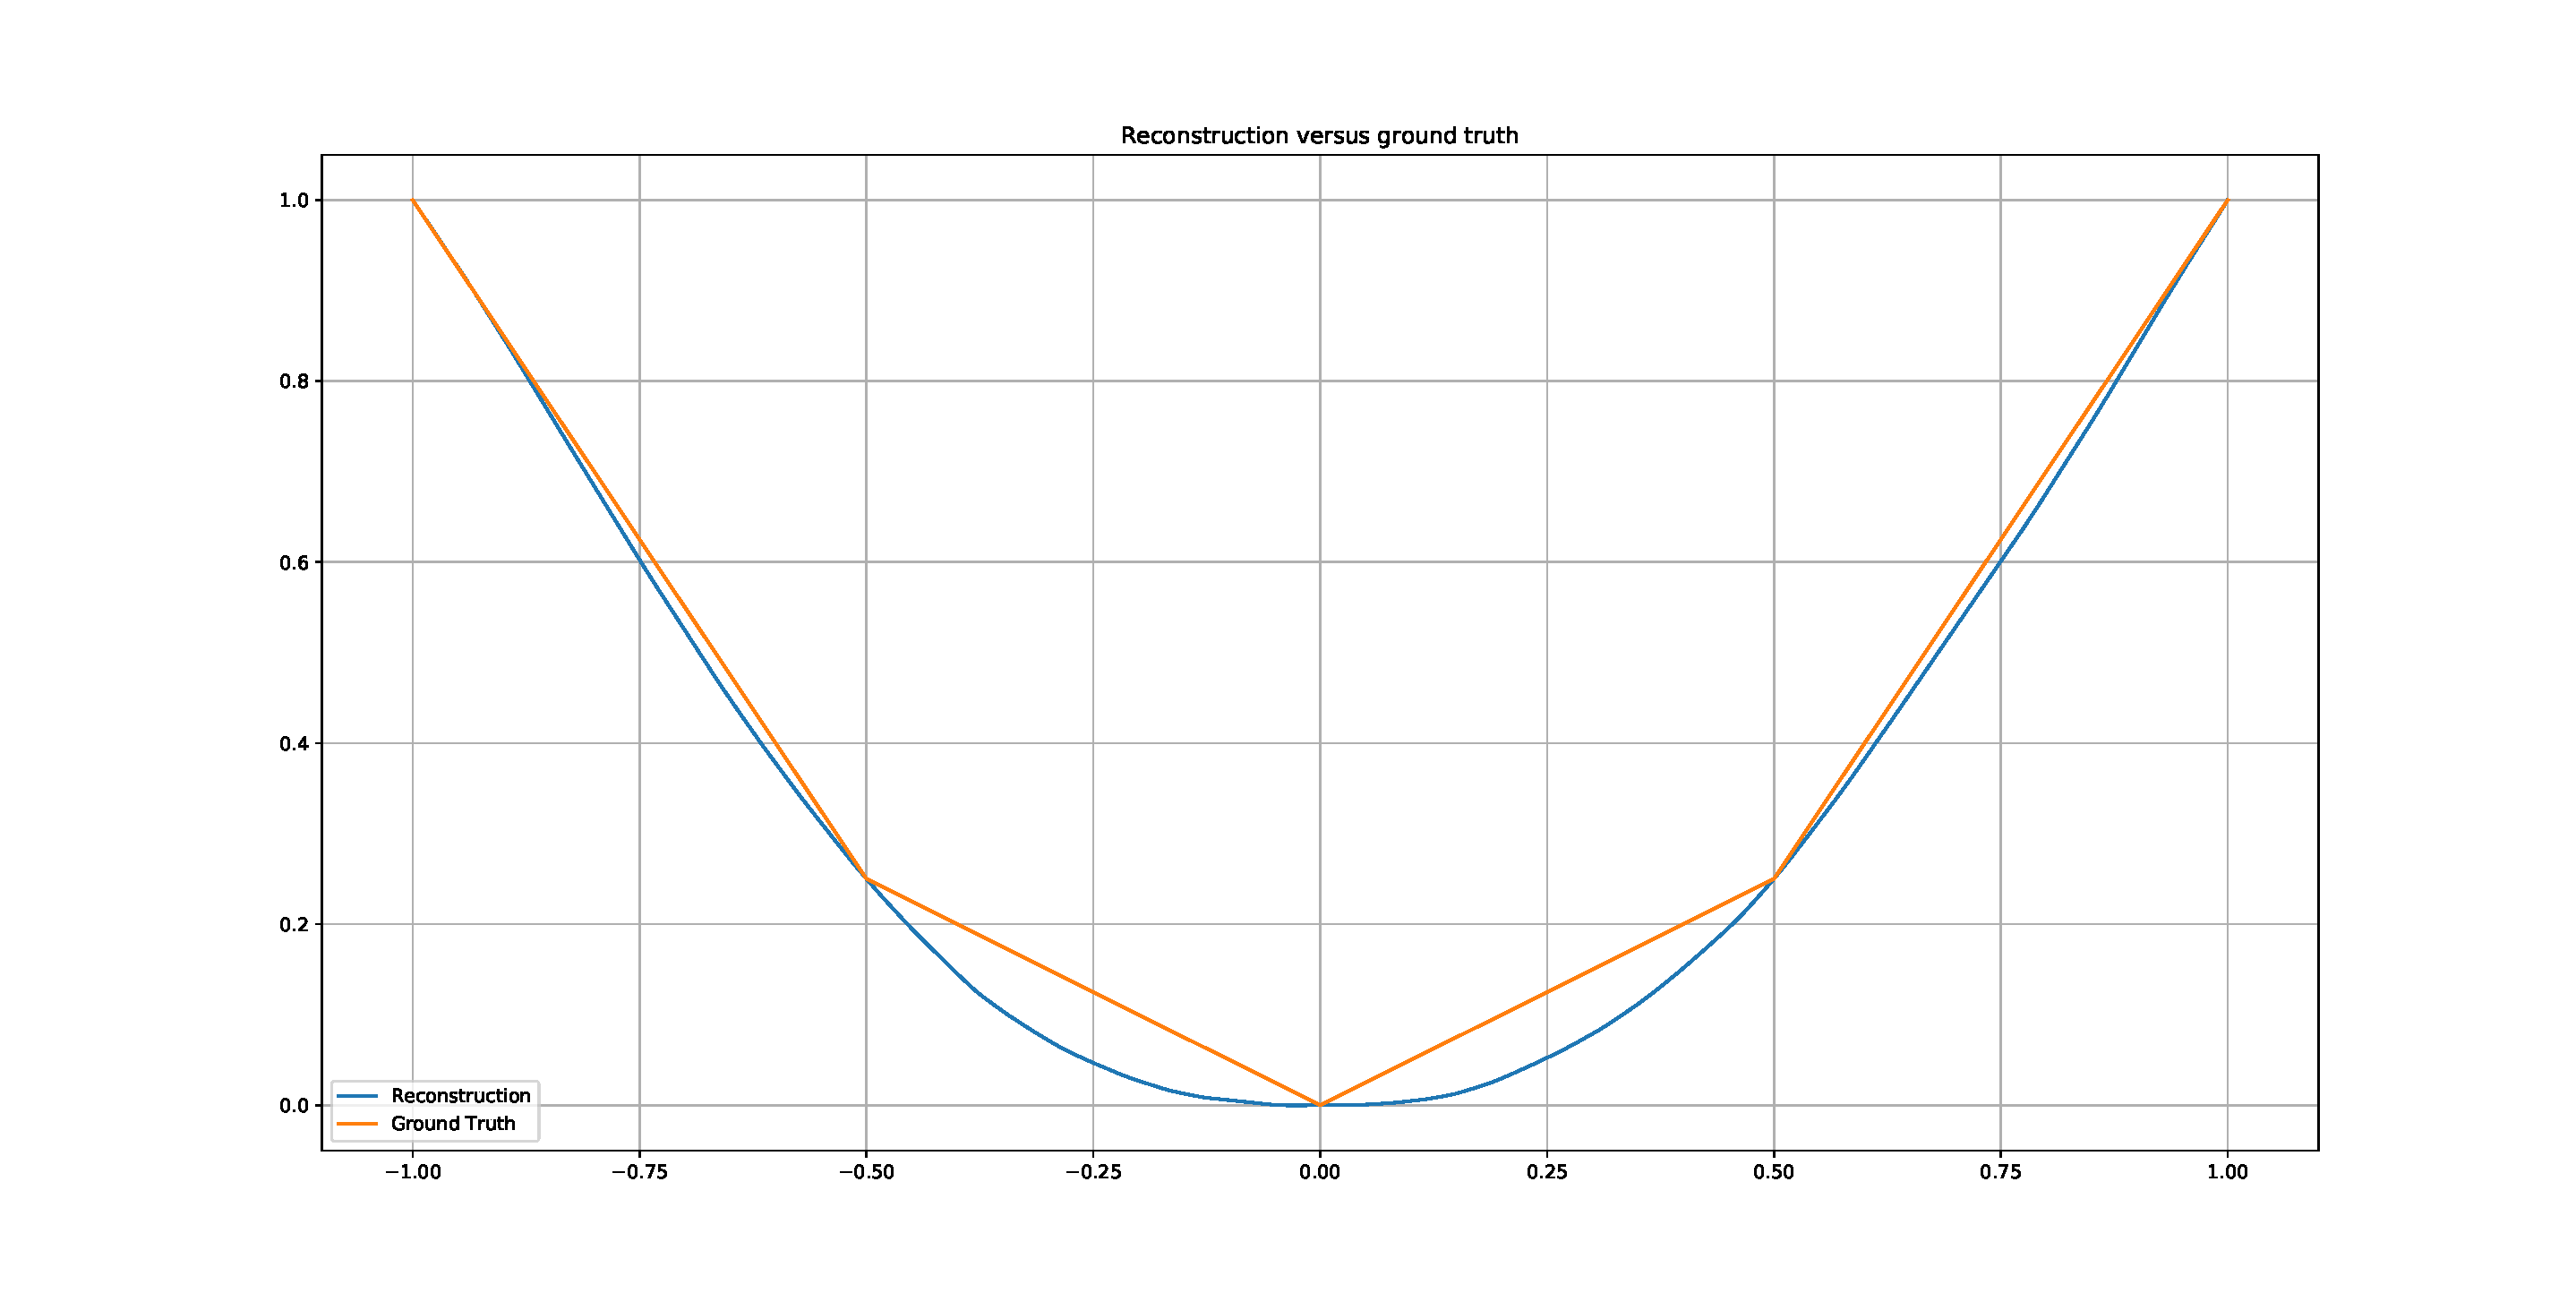
\includegraphics[width=\textwidth]{figures/reconstruction.pdf}
    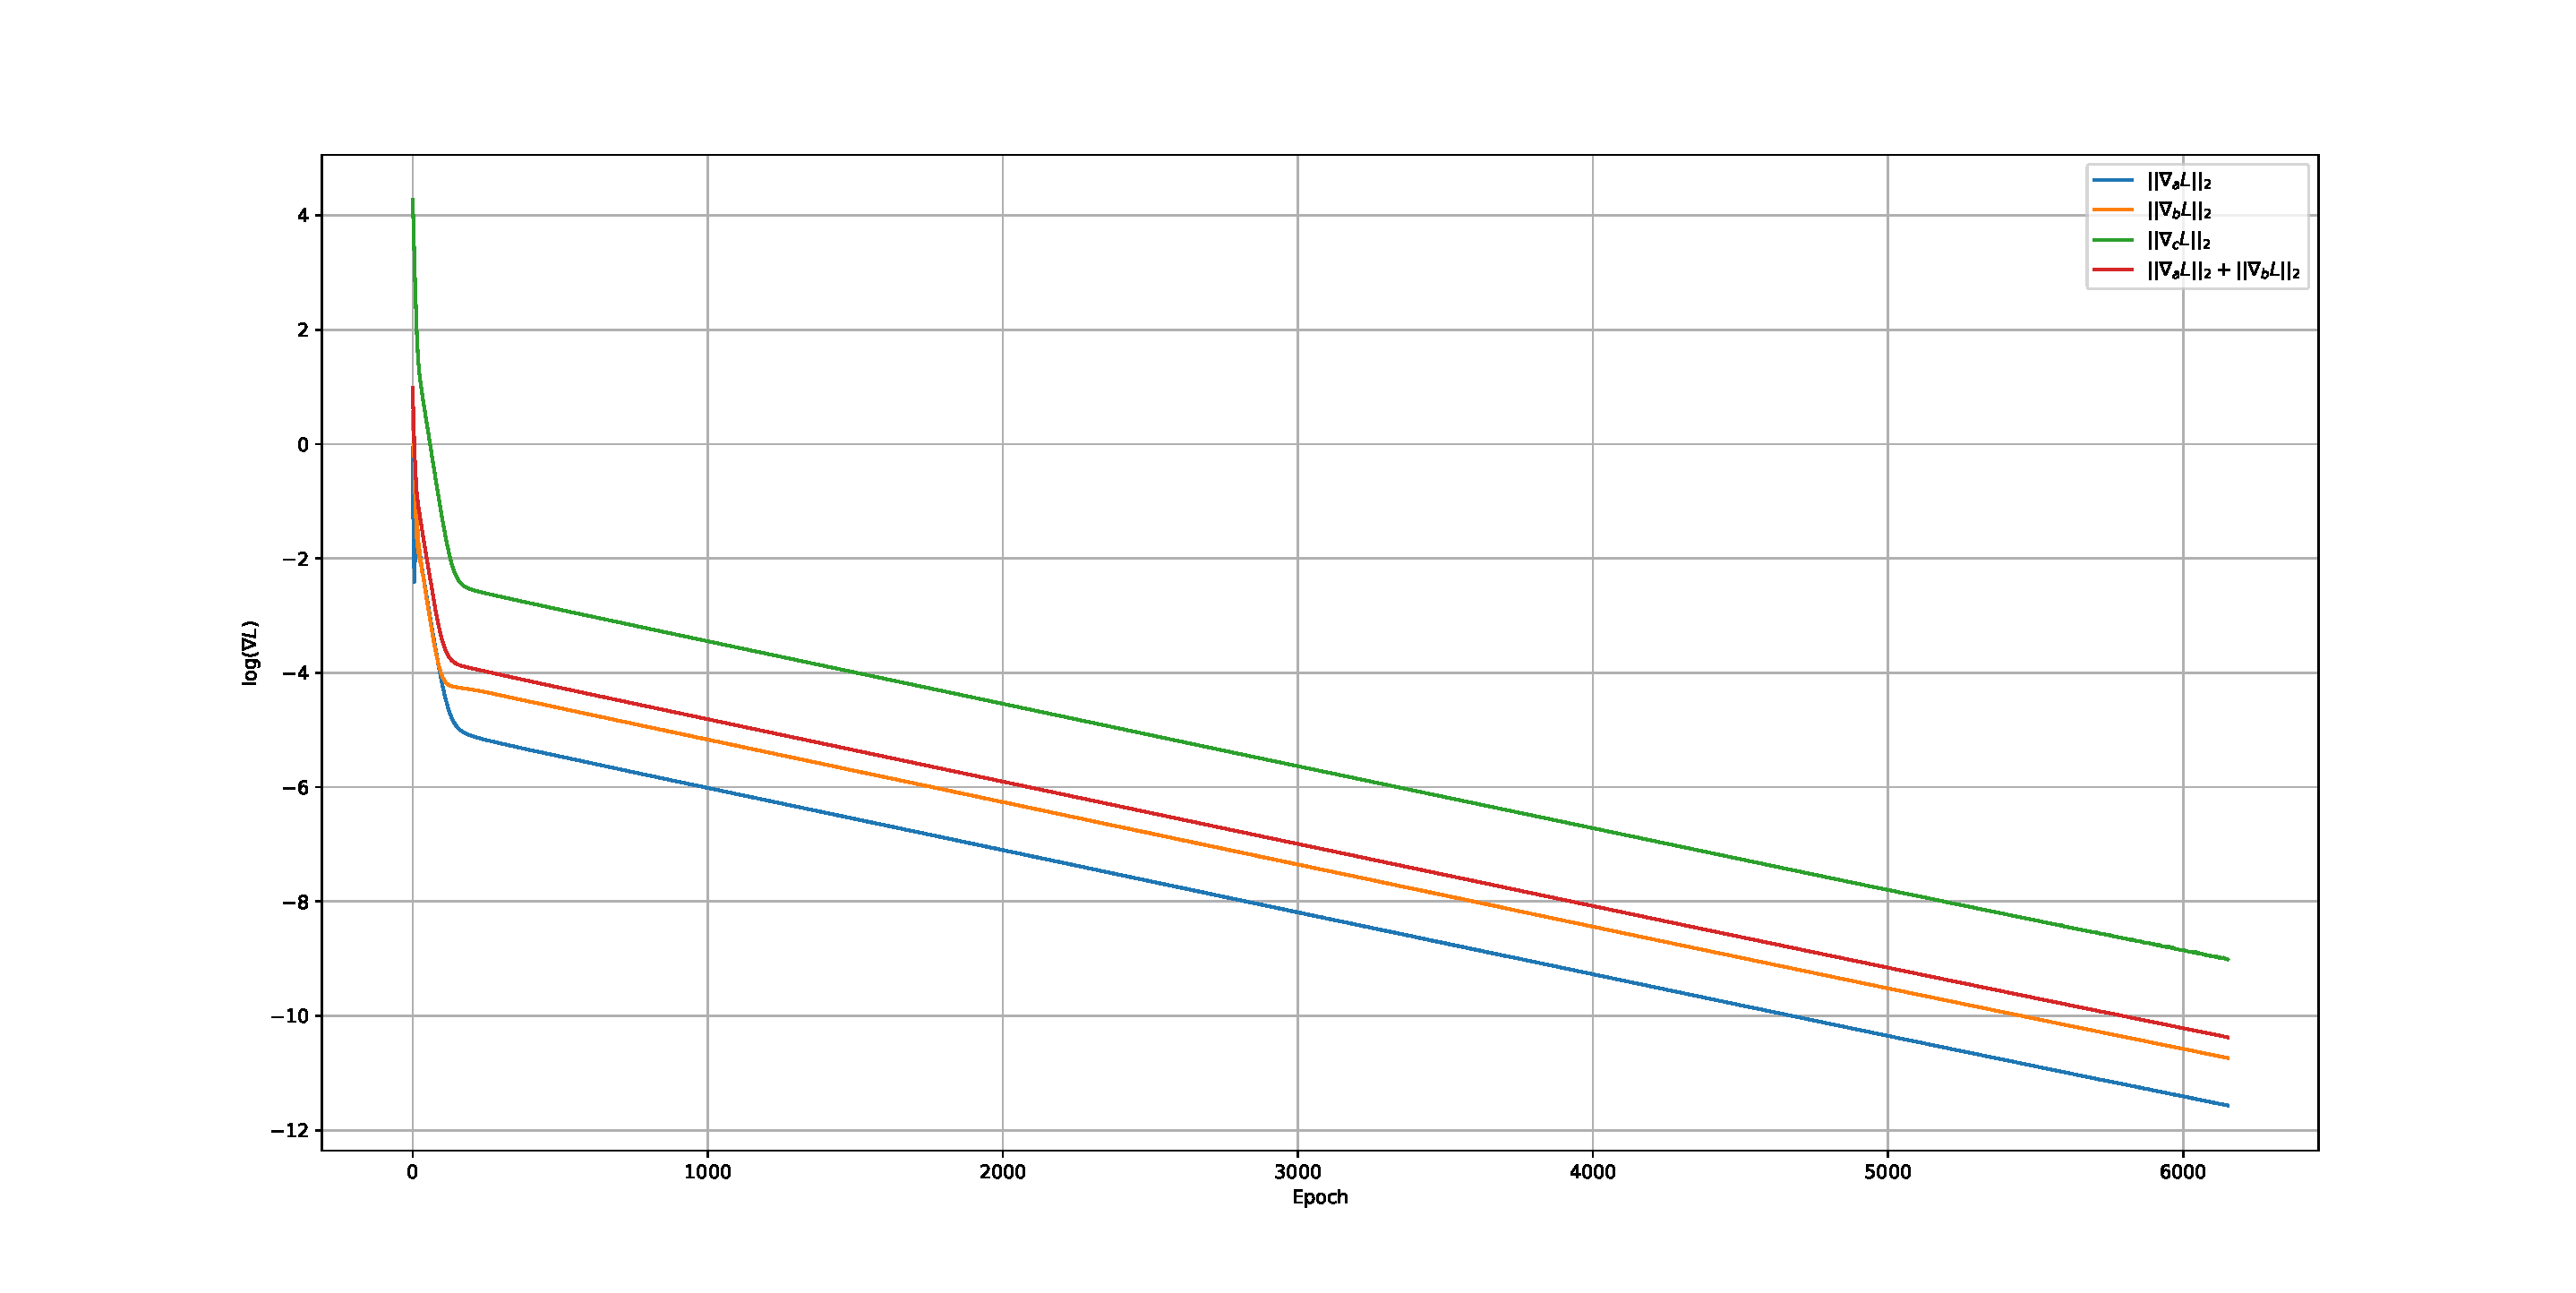
\includegraphics[width=\textwidth]{figures/grad_decay.pdf}
    \caption{Decay of log norms of gradients when  fitting 5 points sampled on the parabola, $y=x^2$ (top). The norm of the gradient $log(||\nabla_c L||_2)$ decays at a slower rate than the gradients, $log(||\nabla_a L||_2)$ and $log(||\nabla_b L||_2)$ as well as the sum, $log(||\nabla_a L||_2 + ||\nabla_b L||_2)$. }
    \label{fig:grad_decay}
\end{figure}


\section{Dynamical properties}


\begin{lemma} During the gradient flow (gradient descent with
infinitesimally small step size) the quantities

\begin{equation}
\delta_i = c_i^2 - \|a_i\|^2 - b_i^2
\end{equation}

remain constant.
\end{lemma}

\begin{proof} This follows from the fact that

\begin{equation}\label{eq:delta_i}
\dot{\delta}_i = c_i \dot{c}_i - \sum_{i=1}^d a_i \dot{a}_i - b_i \dot{b}_i = c_i \nabla_{c_i} L_S - \sum_{j=1}^d a_{ij} \nabla_{a_{ij}} L_S - b_i \nabla_{b_i} L_S = 0
\end{equation}

because

\begin{equation}
\begin{aligned}
& \nabla_{a_{ij}} L_S(\theta) = \sum_{r=1}^s c_{i} x_{rj} \cdot \mathds{1}[\langle a_i, x_r \rangle + b_i \ge 0] (f(\theta,x_r)-y_r),\\
& \nabla_{b_i} L_S(\theta) = \sum_{r=1}^s c_{i} \cdot \mathds{1}[\langle a_i, x_r \rangle + b_i \ge 0](f(\theta,x_r)-y_r),\\ 
& \nabla_{c_{i}} L_S(\theta) = \sum_{r=1}^s [\langle a_i, x_r \rangle + b_i]_+(f(\theta,x_r)-y_r)= \sum_{r=1}^s [\langle a_i, x_r \rangle + b_i](f(\theta,x_r)-y_r) \cdot
\mathds{1} [\langle a_i, x_r \rangle + b_i \ge 0].\\
\end{aligned}
\end{equation}

\end{proof}

At initialization, I would expect $\delta_i < 0$. 

\paragraph{Numerical Experiment}
We check this result numerically for a single layer (1024 neurons) neural network from 1D to 1D. The plot shows the values of $\delta_i$ for each neuron at each iteration in the network:
\begin{figure}[h!]
    \centering
    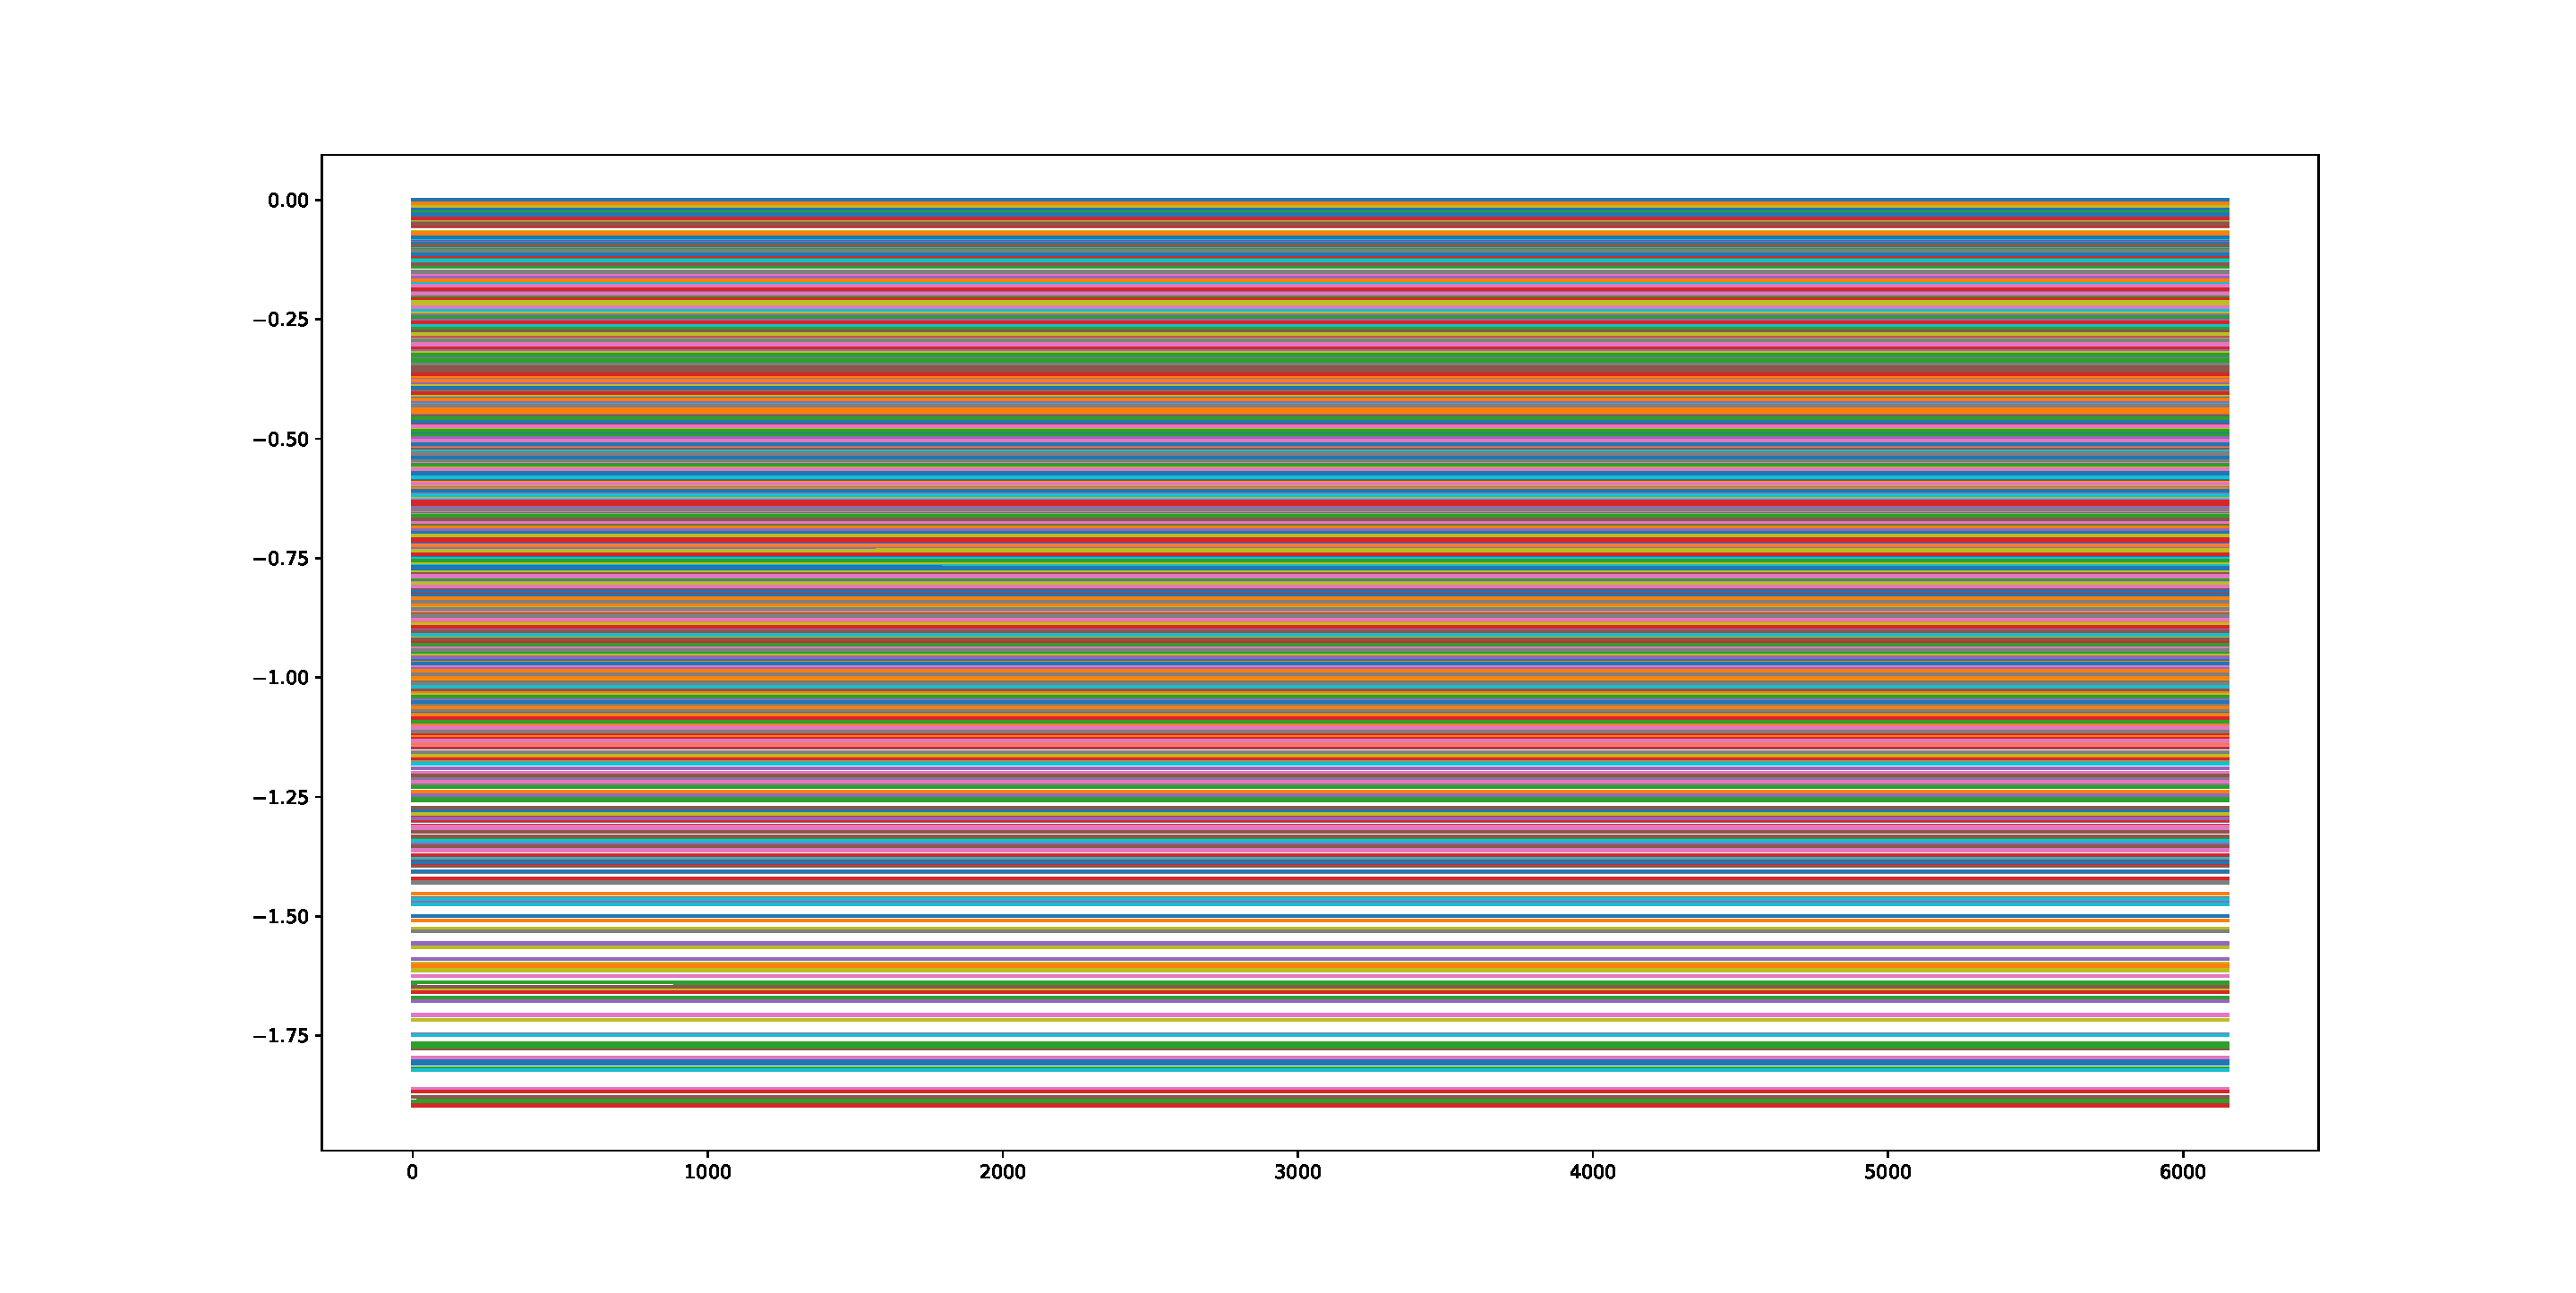
\includegraphics[width=\textwidth]{figures/delta_i.pdf}
    \caption{The evolution of the $\delta_i$s as the optimization proceeds. The $x$ axis is iterations and each colored line corresponds to an individual $\delta_i$. Note how all the $\delta_i$ are roughly consntant and negative.} 
    \label{fig:my_label}
\end{figure}

We sample $\delta_i$ at each iteration, yielding $\delta_i[1], \ldots \delta_i[N]$. The maximum and minimum divergences between $\delta_i$ and its mean are:
\begin{align*}
\max_i \max_j \bigg|\delta_i[j] - \frac{1}{N}\sum_{j=1}^N \delta_i[j]\bigg| &= 0.00019788742 \\
\min_i \max_j \bigg|\delta_i[j] - \frac{1}{N}\sum_{j=1}^N \delta_i[j]\bigg| &= 5.5879354\times10^{-9}
\end{align*}

\section{Removing overparameterization}

We define a \emph{minimal ReLU network} as a function of the form

\begin{equation}
g(\xi, x) = \sum_{i=1}^{m} \varepsilon_i [\langle u_i, x \rangle + v_i]_+, \quad s_i \in \{+, - \}, \quad \xi=((\varepsilon_i,u_i,v_i))
\end{equation}

Every shallow ReLU network with at most \(m\) neurons can be written in
this form. The new parameterization eliminates \(m\) degrees of freedom.
The association between parameters is simply

\begin{equation}
(c_i,a_i,b_i) \mapsto (sign(c_i), |c_i| a_i, |c_i| b_i).
\end{equation}


\end{document}